

\begin{figure}[htbp]
    \centering
    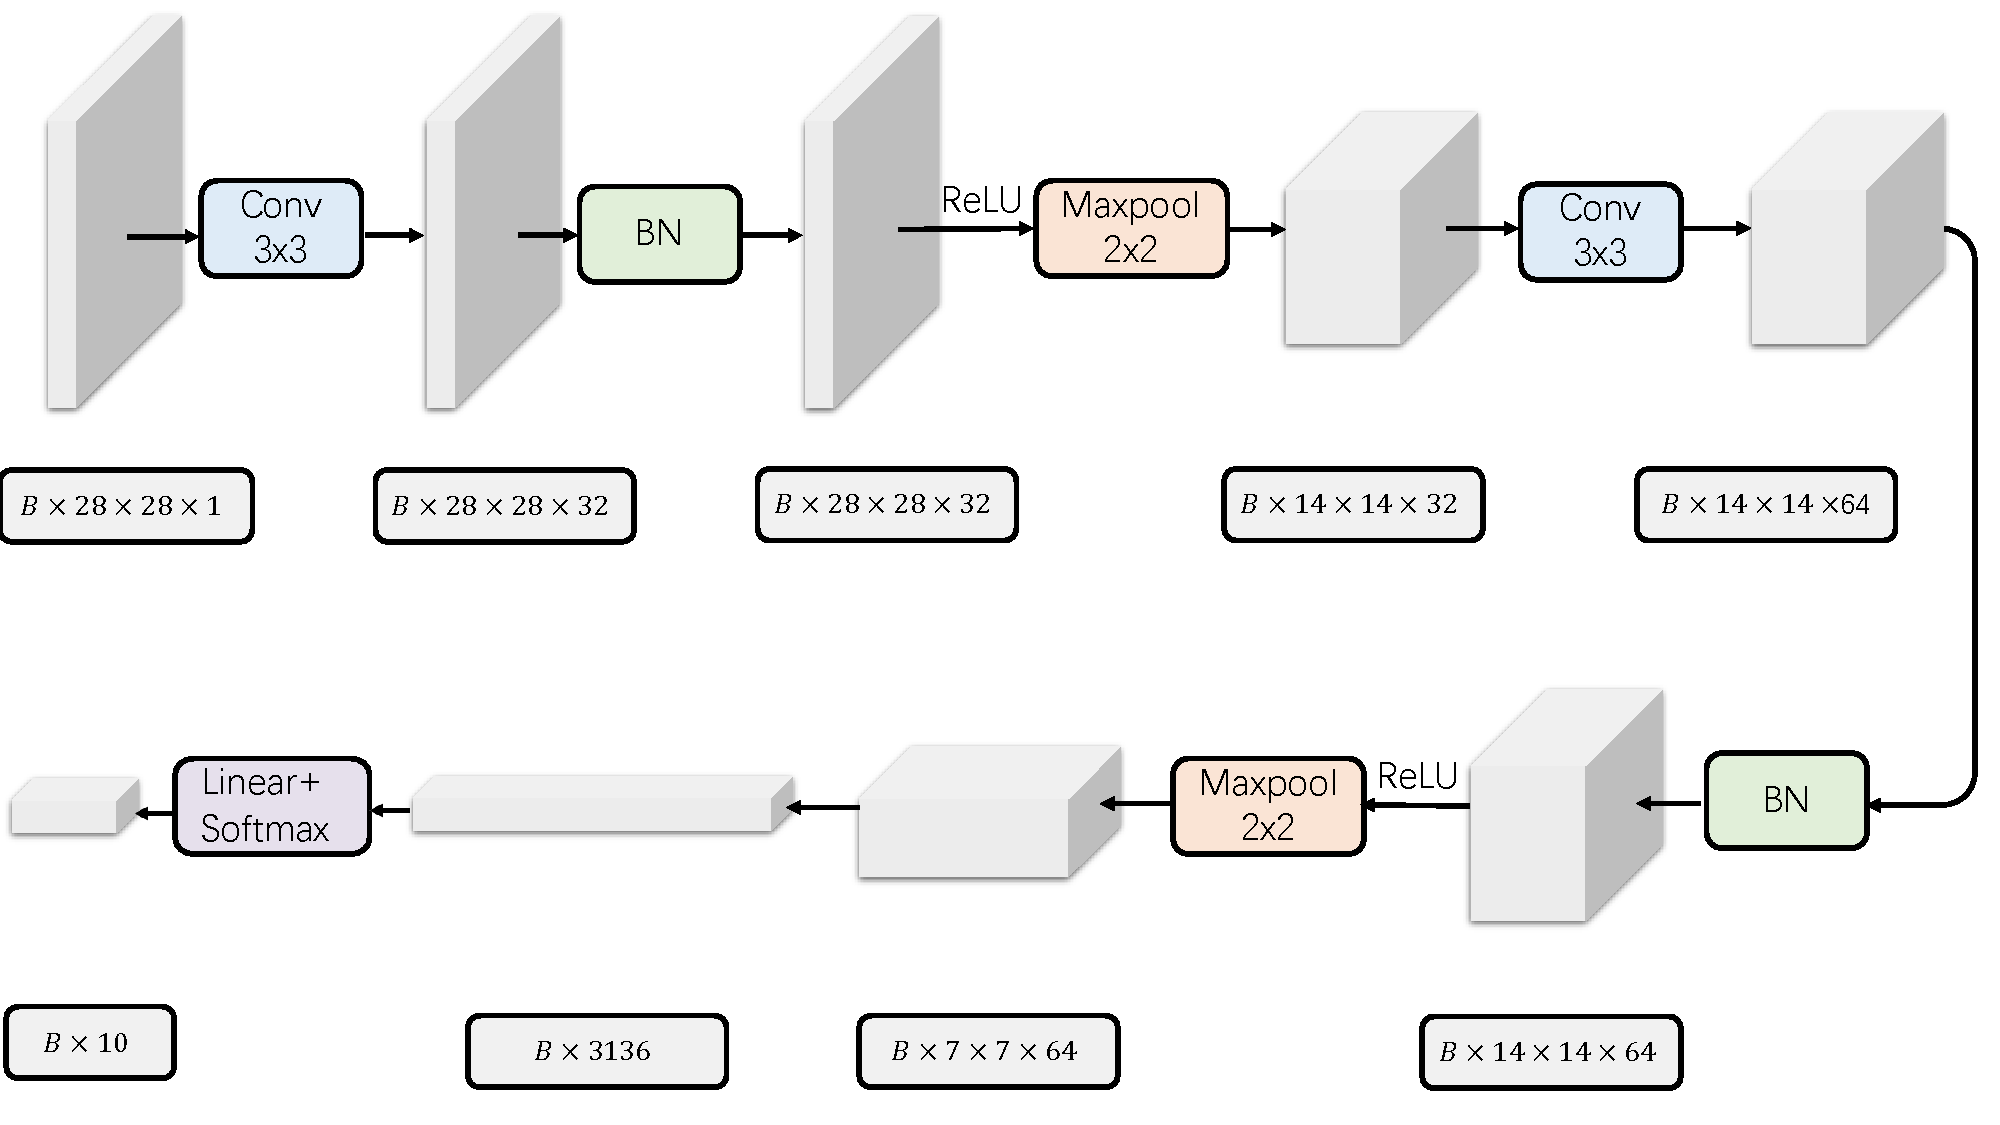
\includegraphics[width=0.8\textwidth]{cnn.pdf}
    \caption{Model diagram of self-designed CNN network for MNIST image classification task. The whole model contains 12 neural layers including the output layer. $B$ stands for the size of a batch.}
    \label{fig:CNN_arch}
\end{figure}

\begin{figure}[htbp]
    \centering
    \includegraphics[width=0.9\textwidth]{../images/mnist-train-loss-acc.png}
    \caption{Training loss and accuracy change figures. The left figure corresponds to the change of loss and the right one corresponds to the change of accuracy.}
    \label{fig:cnn_loss_acc}
\end{figure}

\begin{figure}[htbp]
    \centering
    \begin{subfigure}
        \centering
        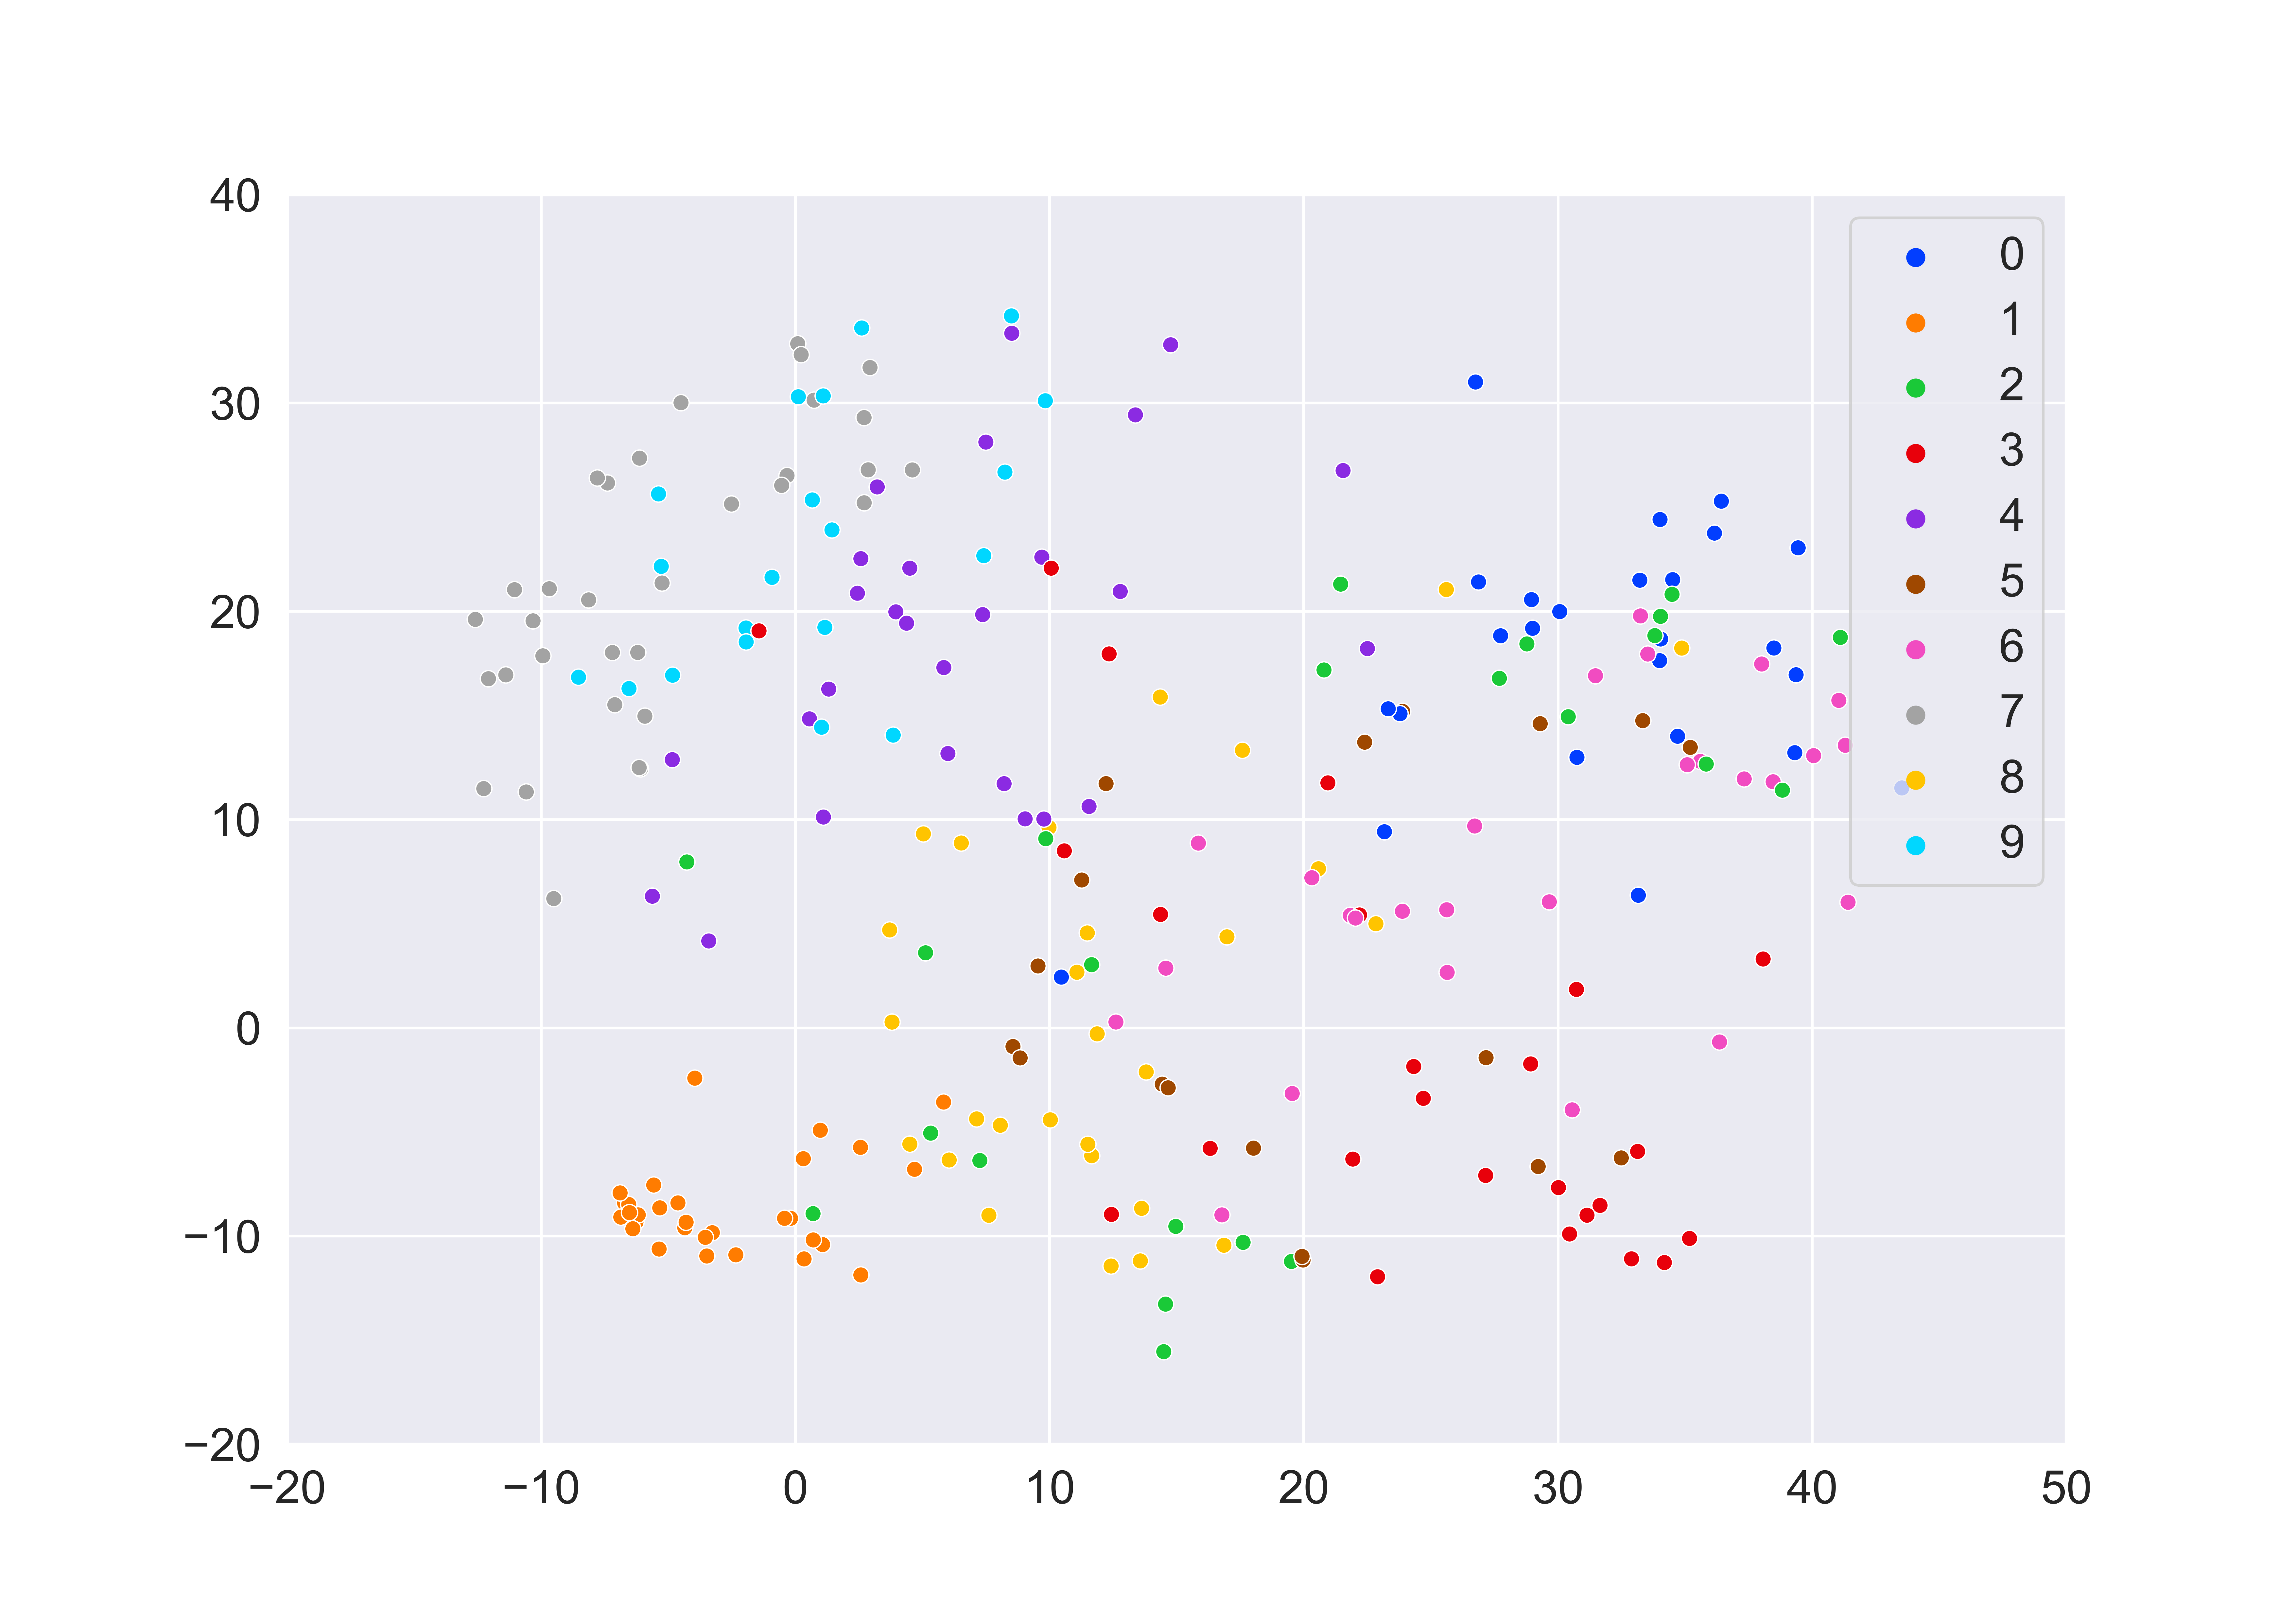
\includegraphics[width=0.32\linewidth]{../images/mnist_feature_map1_pca.png}
        % \caption{a}
        \label{fig:mnist_pca_1}
    \end{subfigure}
    % \hfill 
    \begin{subfigure}
        \centering
        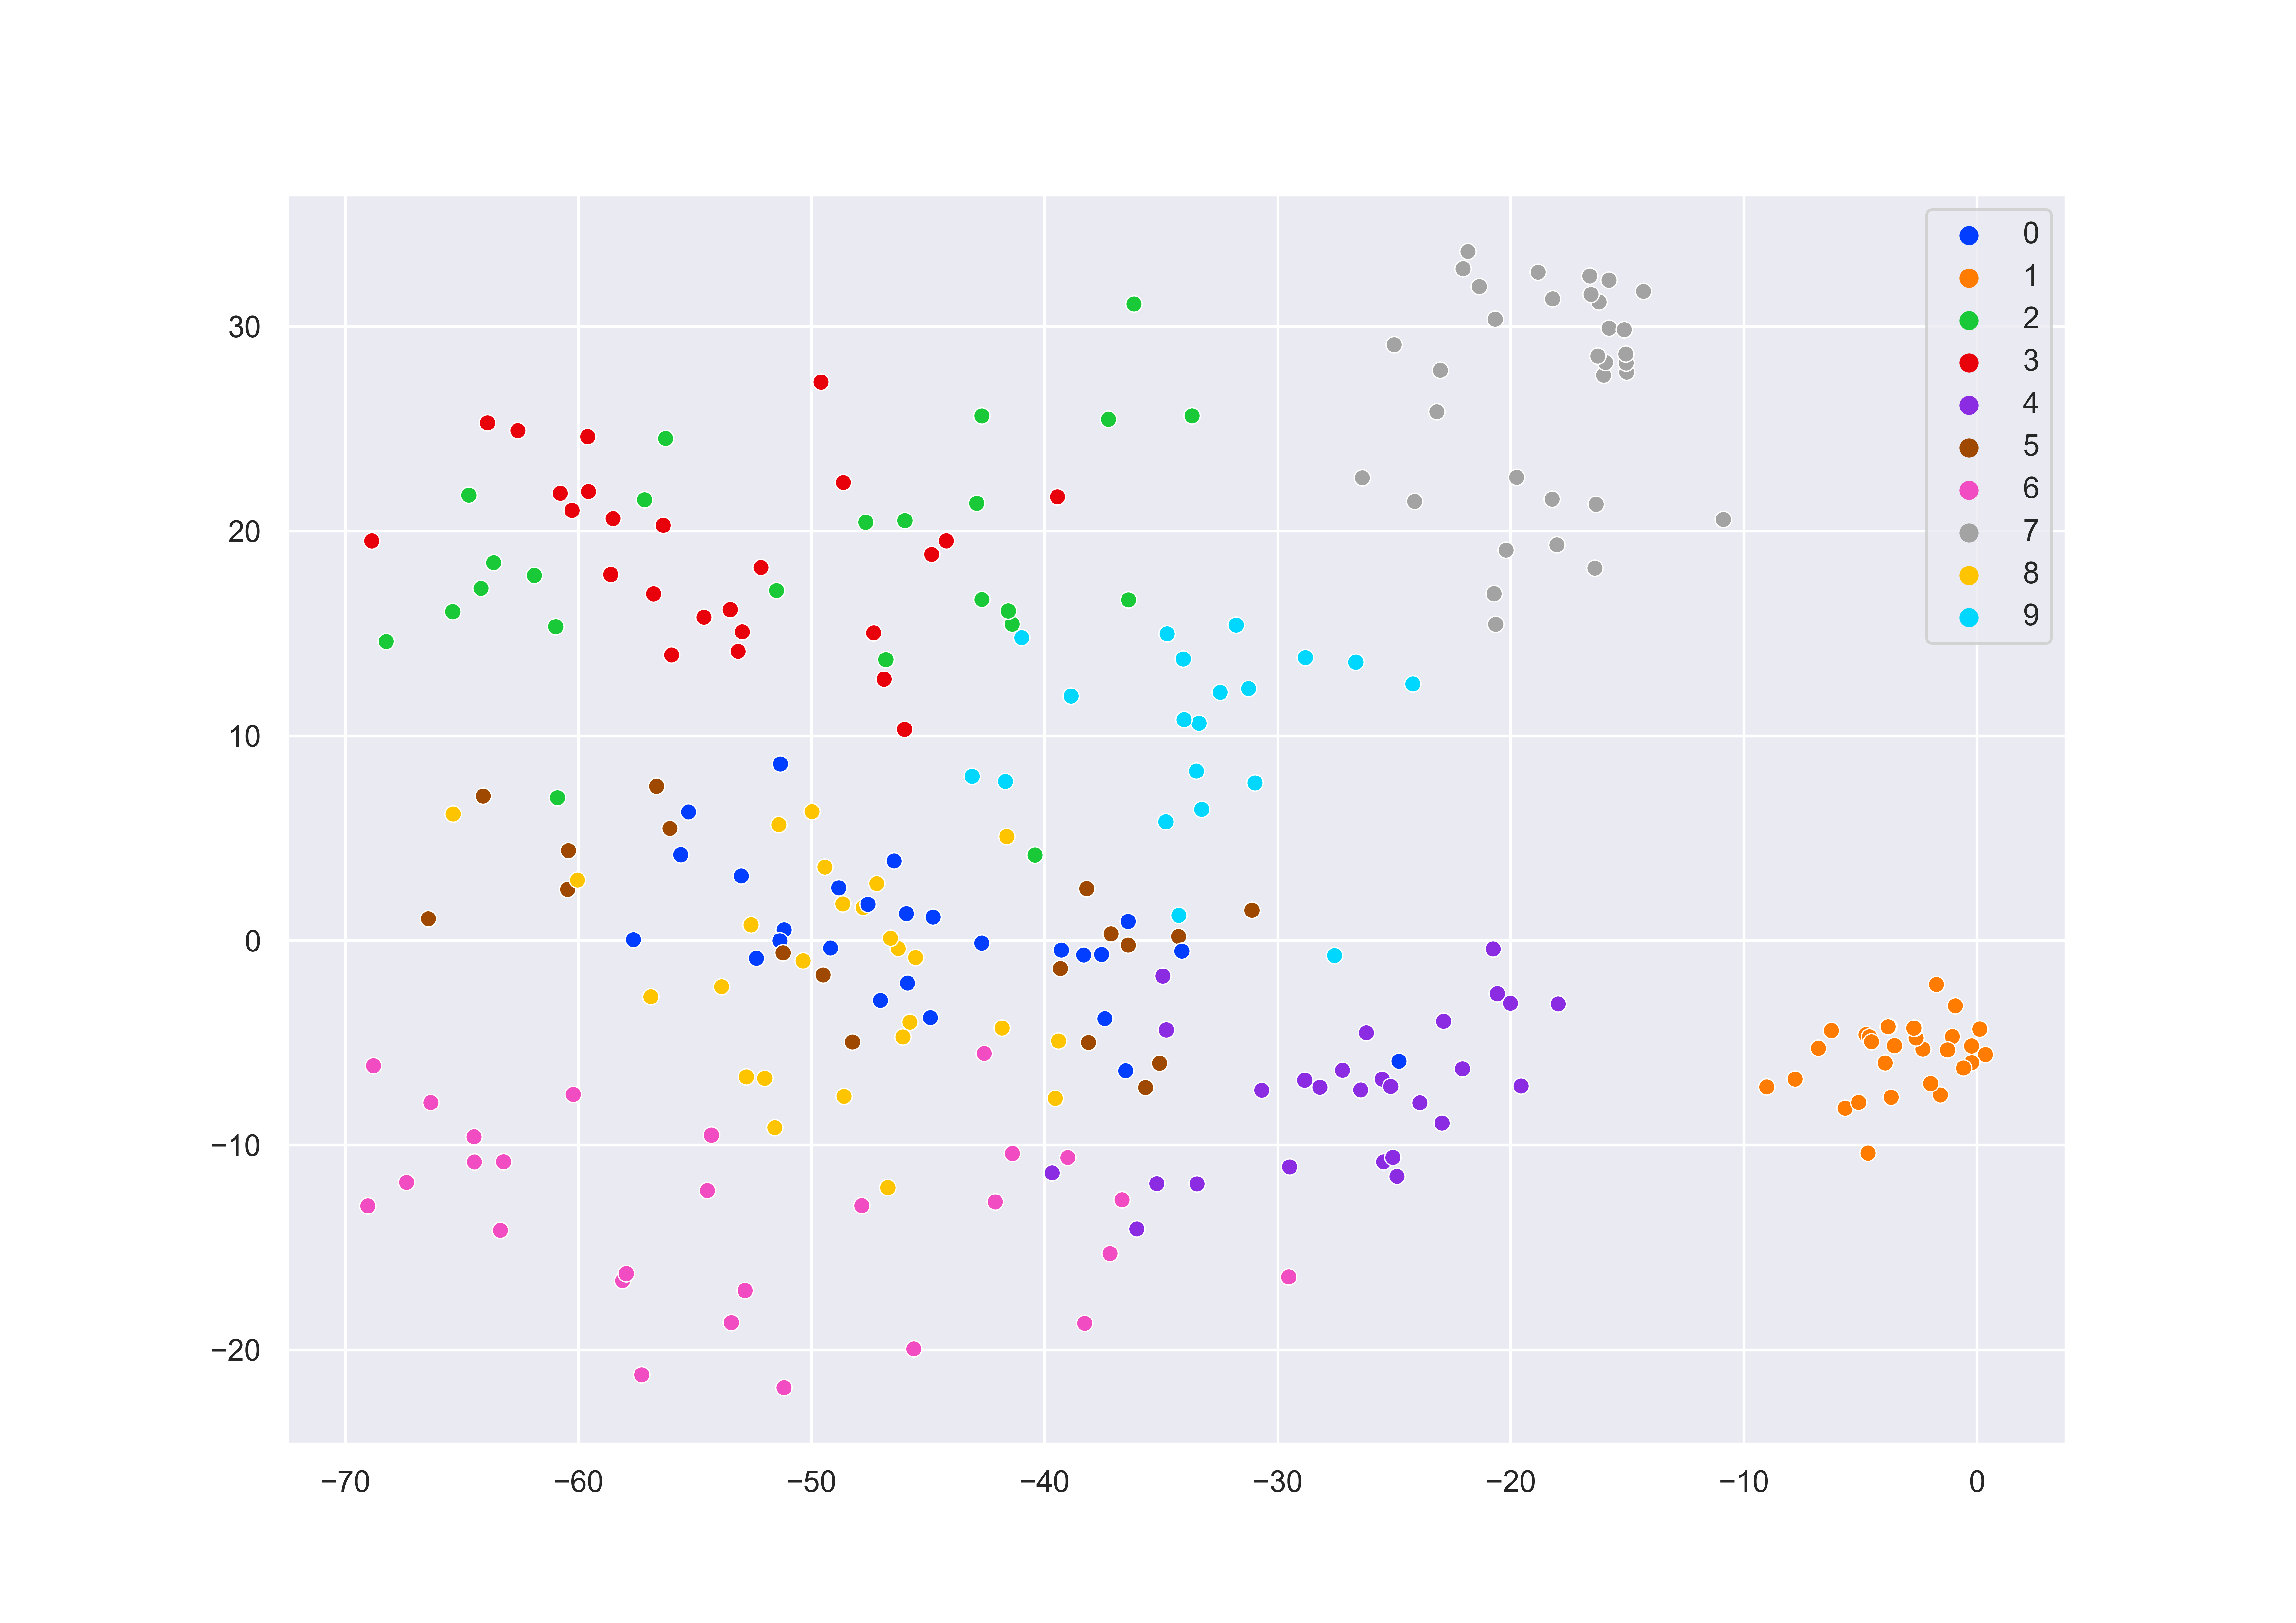
\includegraphics[width=0.32\linewidth]{../images/mnist_feature_map2_pca.png}
        % \caption{Absolute value of indivisual components of weight in ridge regression when setting $\lambda$ to 1.0.}
        \label{fig:mnist_pca_2}
    \end{subfigure}
    % \hfill 
    \begin{subfigure}
        \centering
        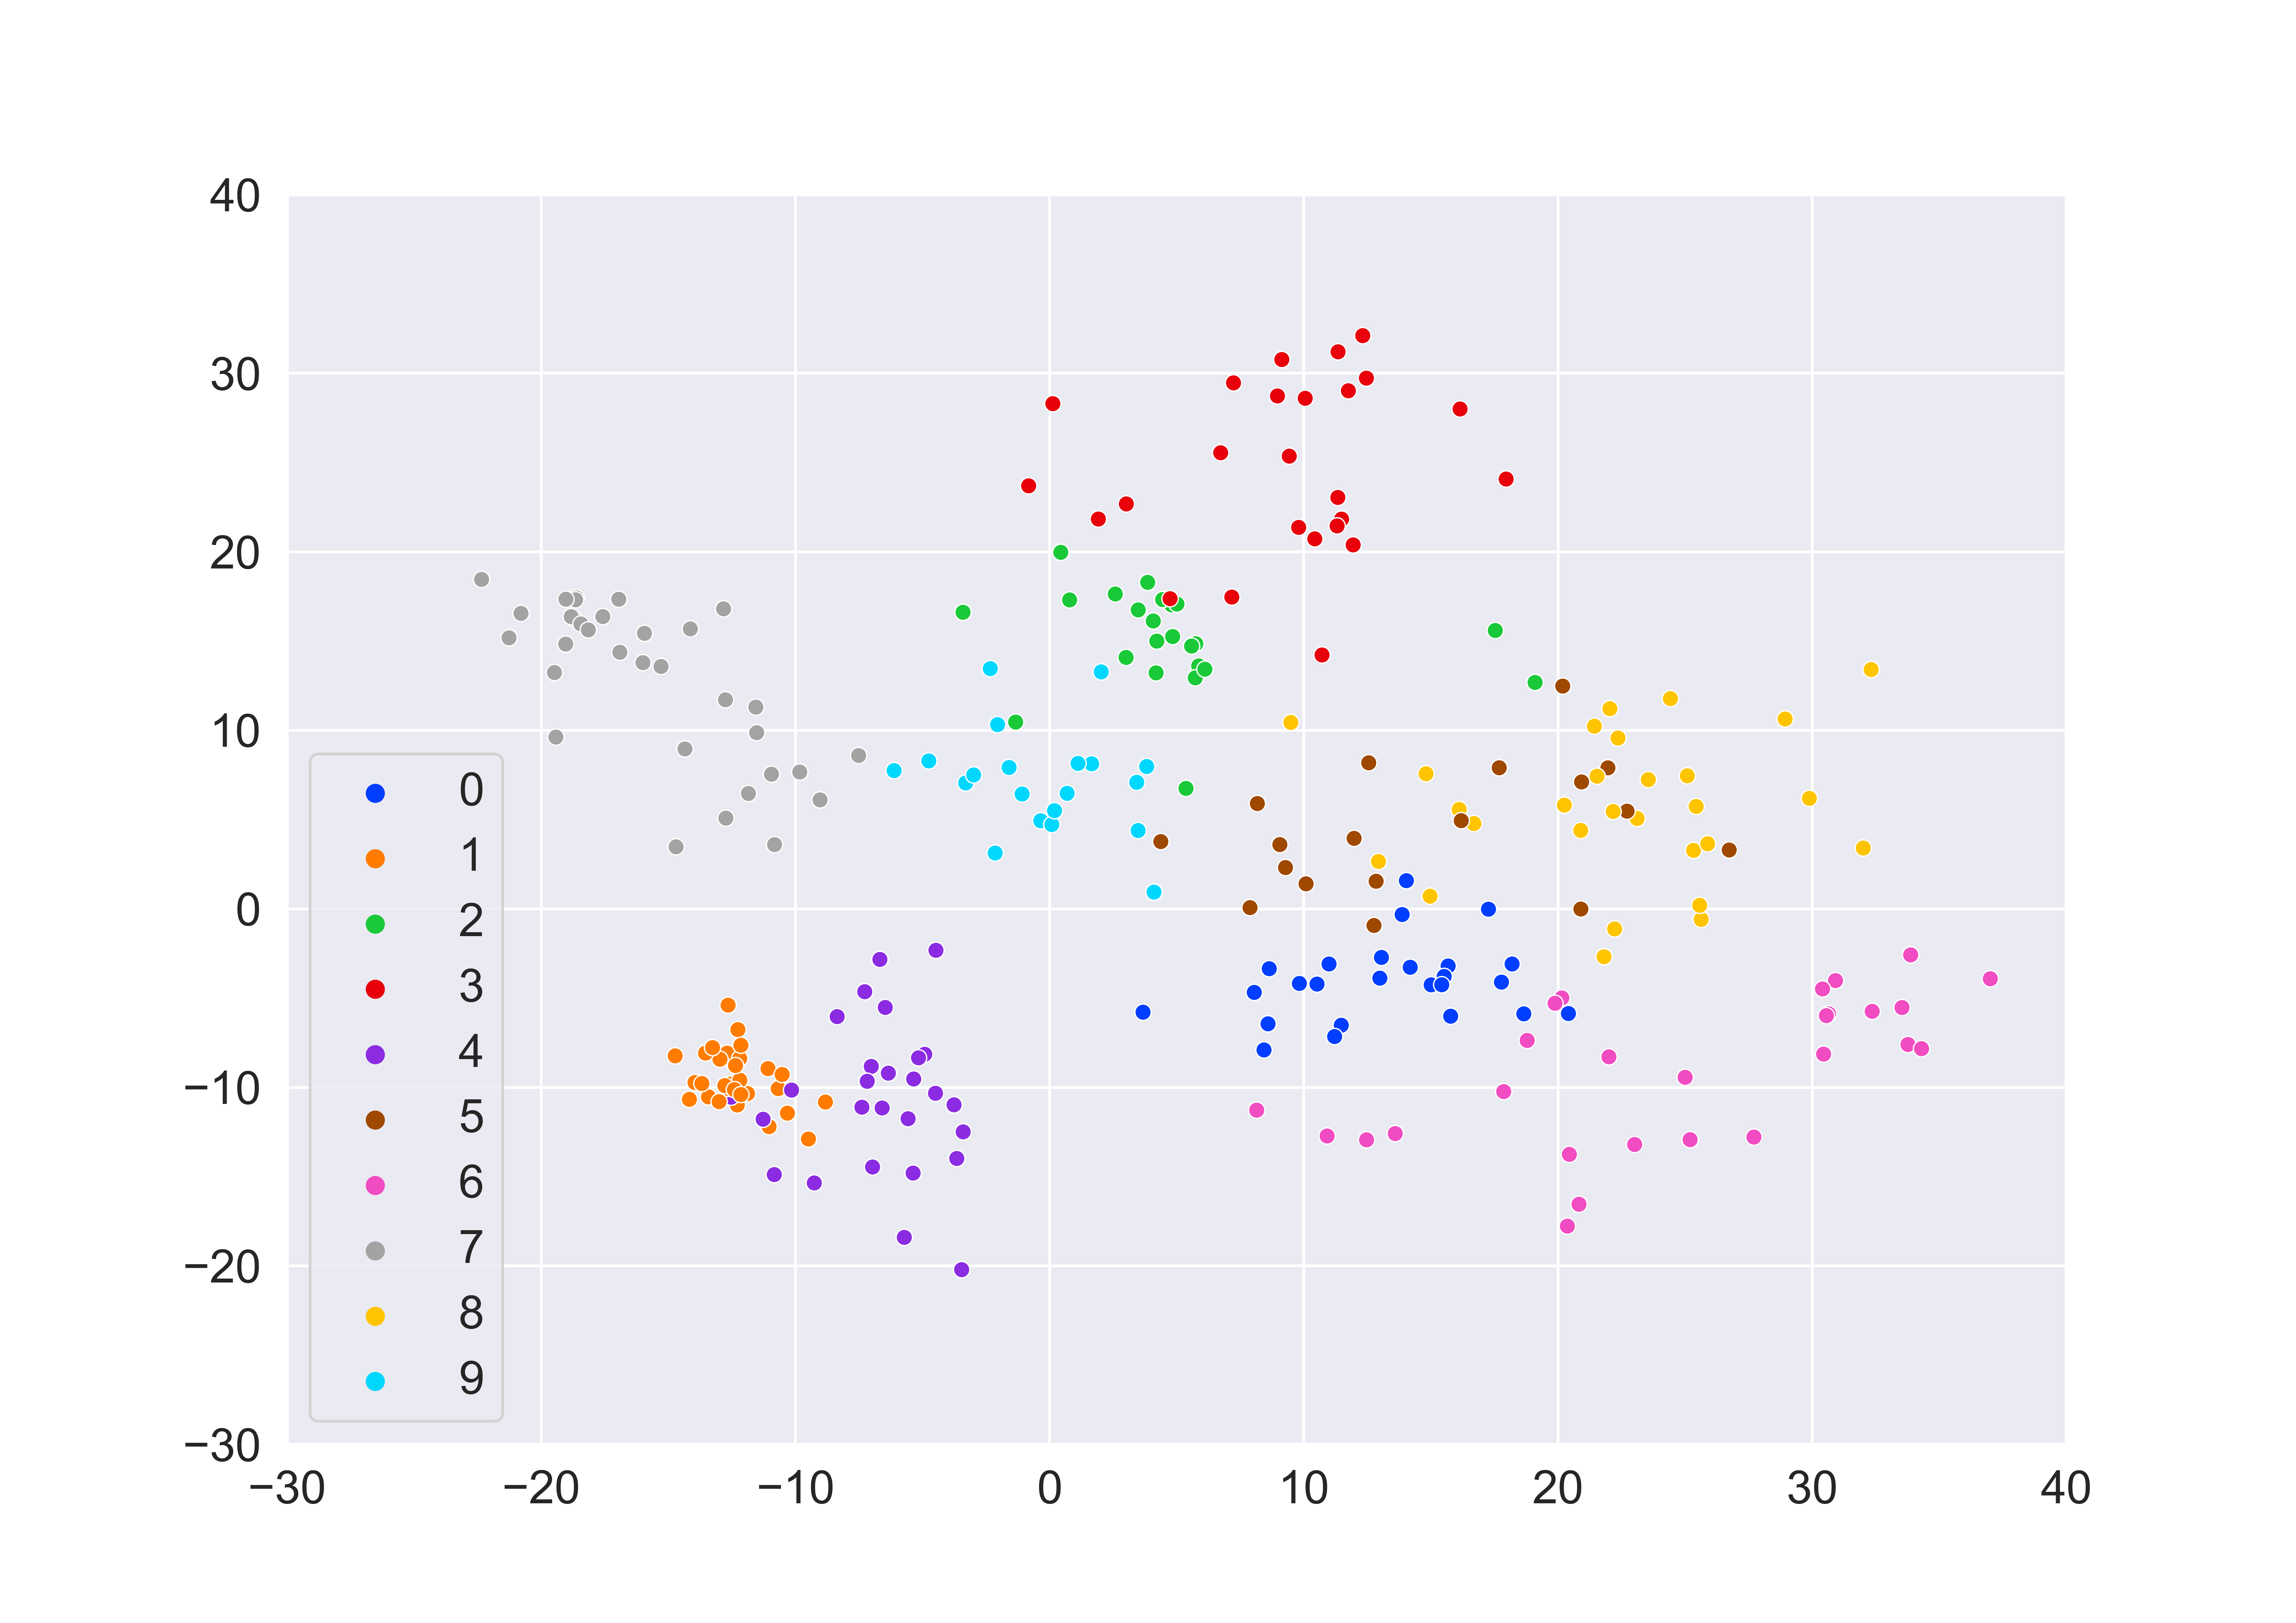
\includegraphics[width=0.32\linewidth]{../images/mnist_feature_map3_pca.png}
        % \caption{Absolute value of indivisual components of weight in ridge regression when setting $\lambda$ to 1.5.}
        \label{fig:mnist_pca_3}
    \end{subfigure}
    \caption{Visualization images of intermediate output tensors with PCA method. Left: Tensors after the first max pooling layer. Middle: Tensors after the second max pooling layer. Right: Tensors after the output linear layer.}
    \label{fig:mnist_pca}
\end{figure}

\begin{figure}[htbp]
    \centering
    \begin{subfigure}
        \centering
        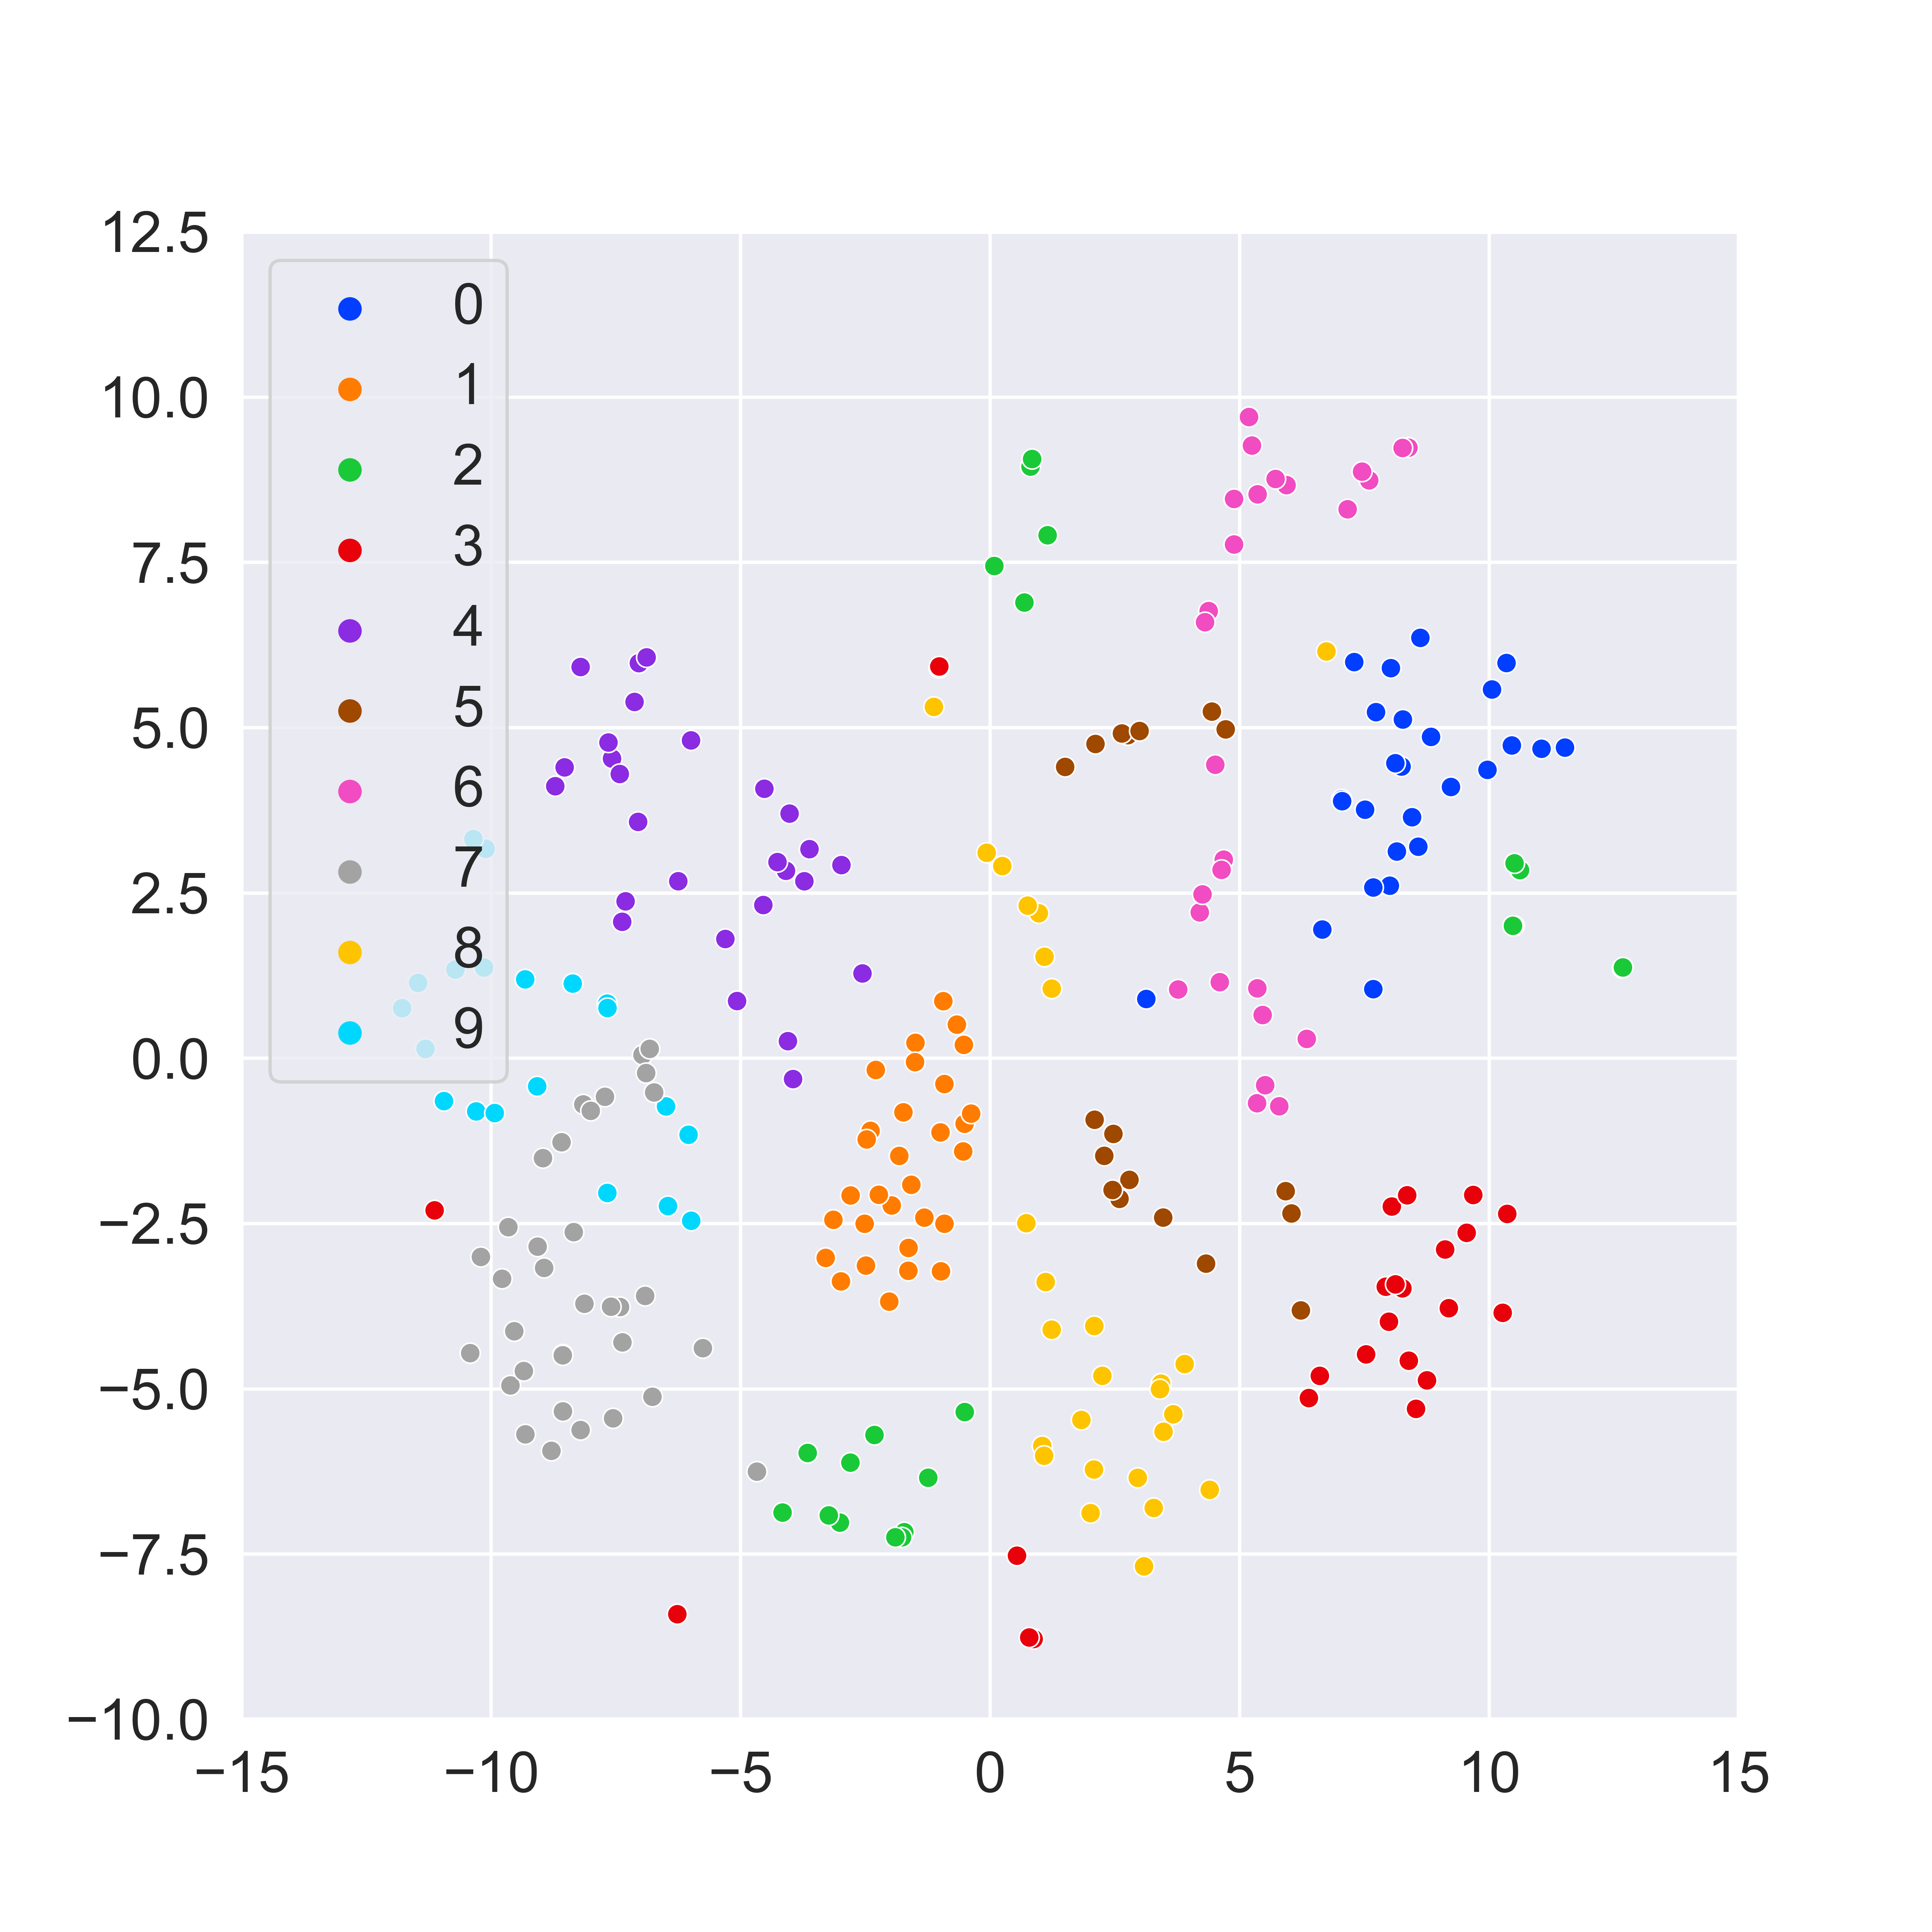
\includegraphics[width=0.32\linewidth]{../images/mnist_feature_map1_tsne.png}
        % \caption{a}
        \label{fig:mnist_tSNE_1}
    \end{subfigure}
    % \hfill 
    \begin{subfigure}
        \centering
        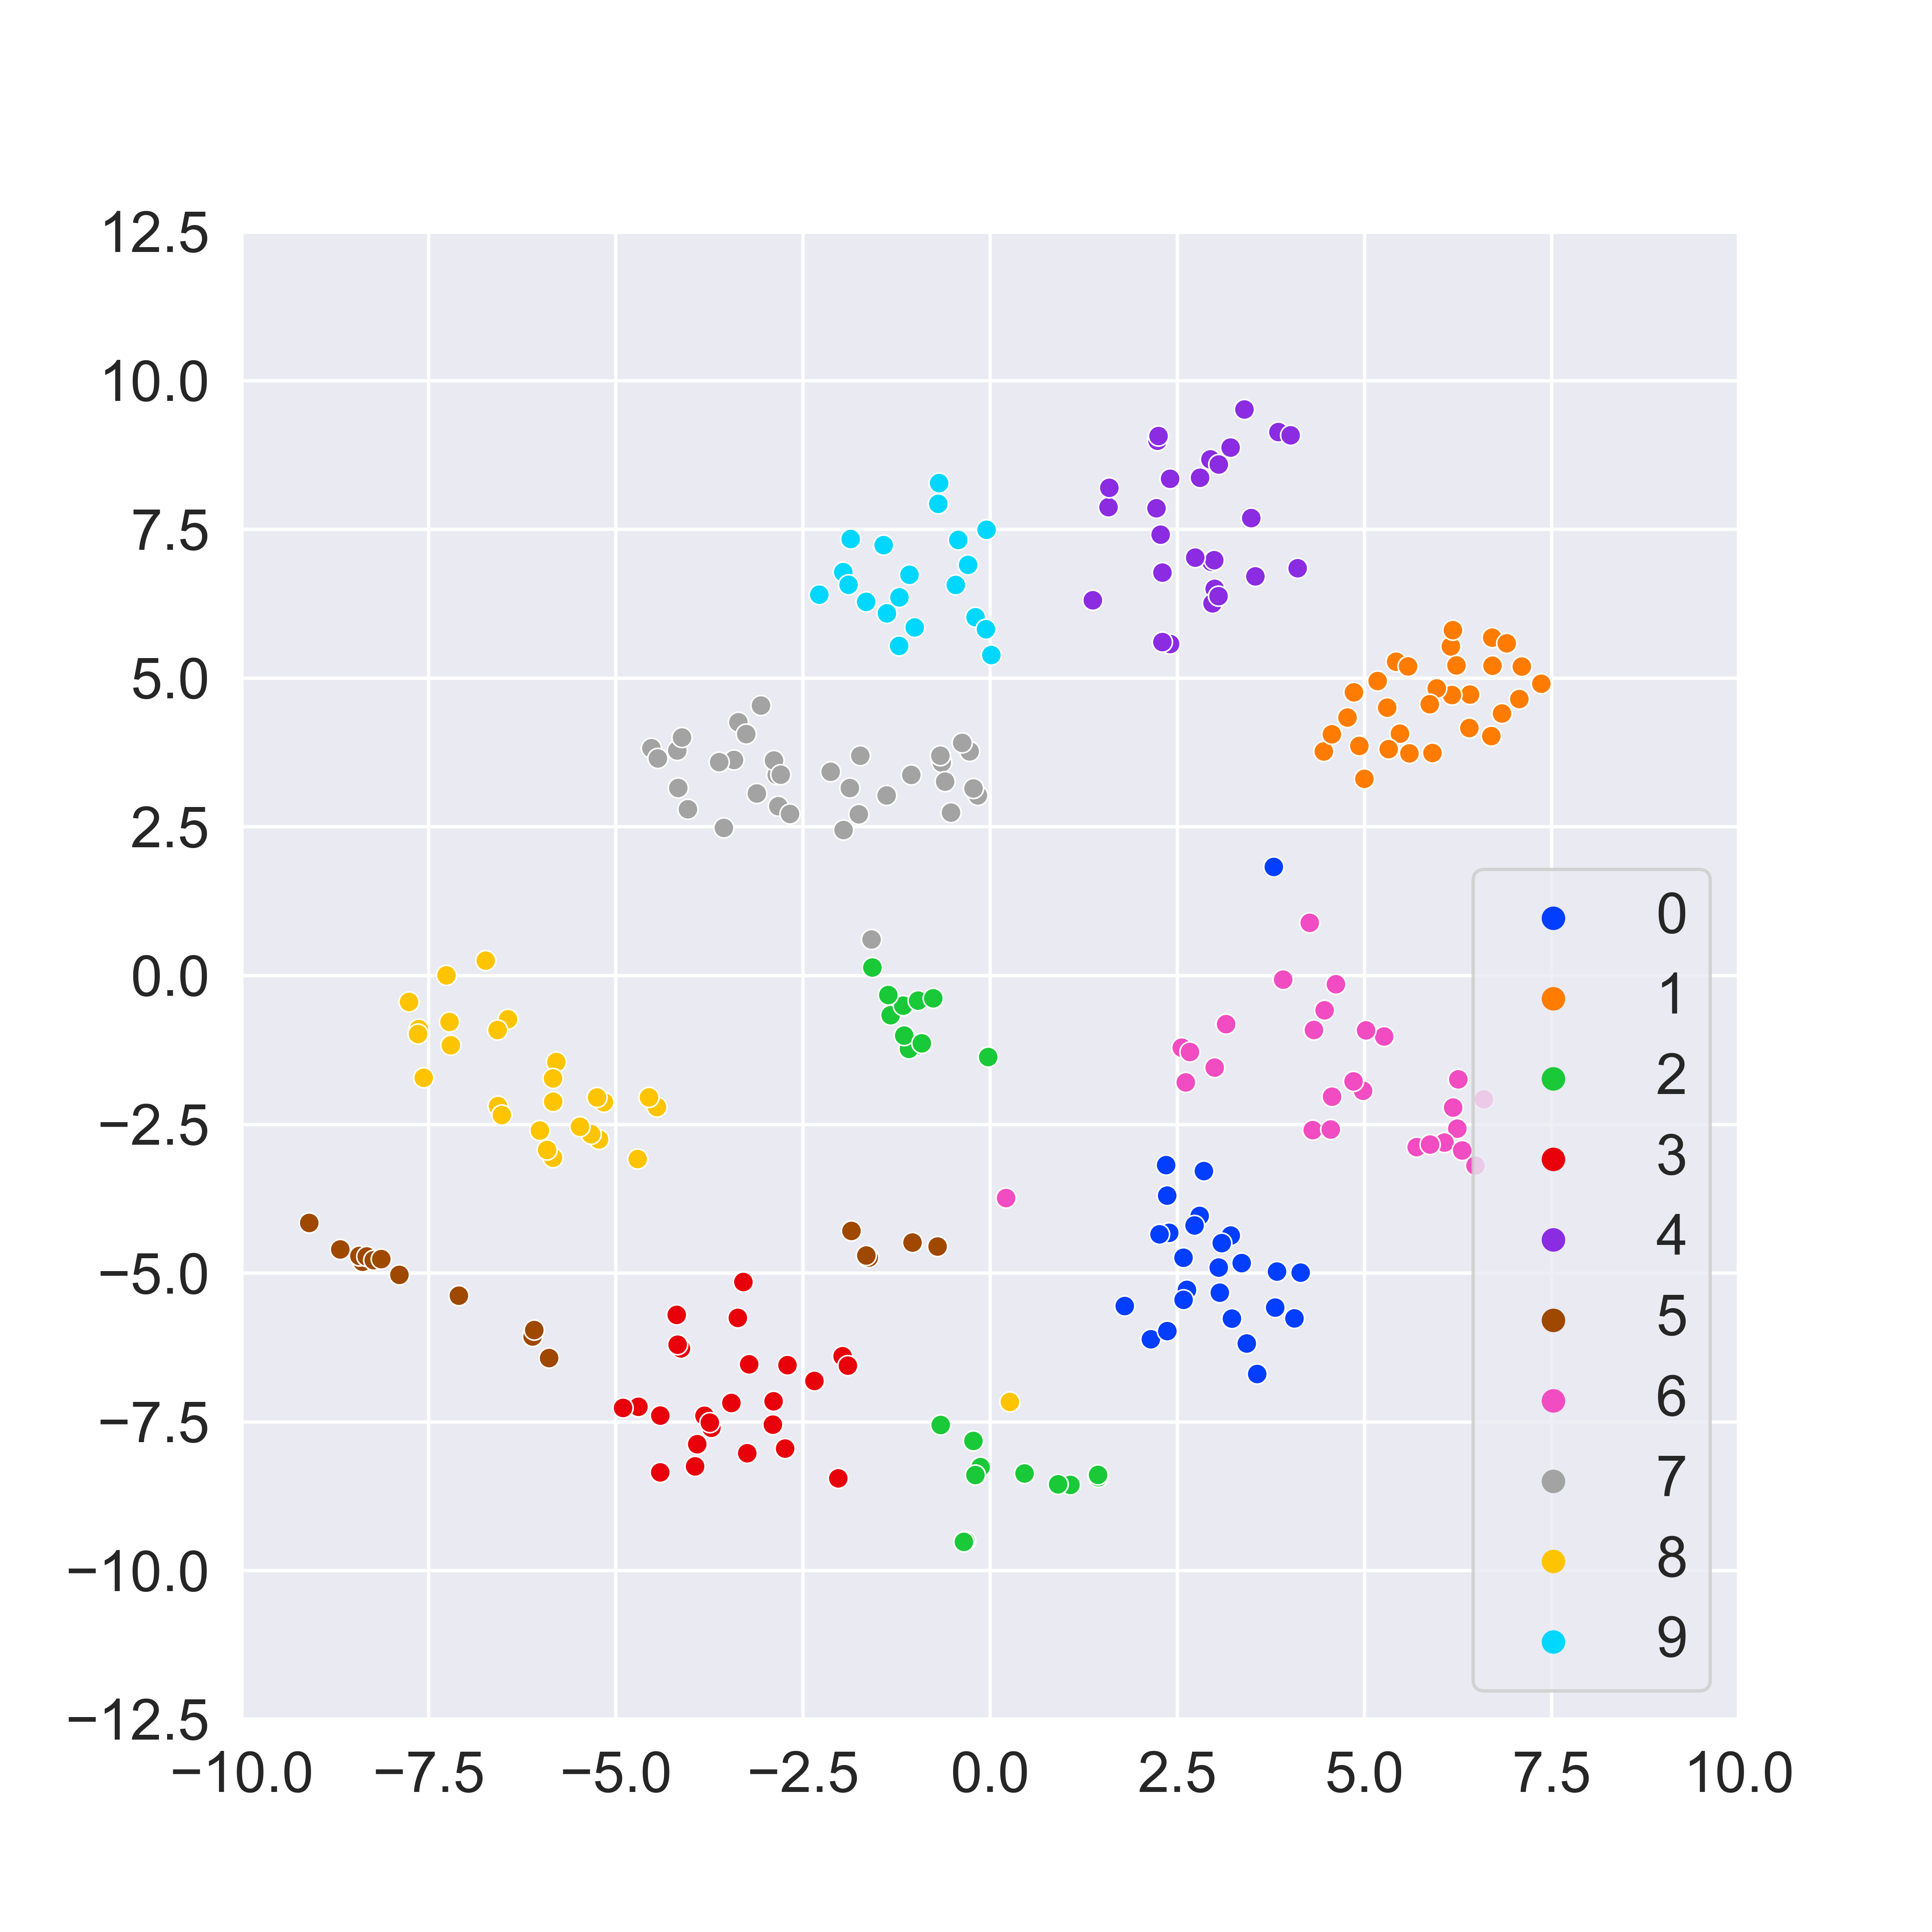
\includegraphics[width=0.32\linewidth]{../images/mnist_feature_map2_tsne.png}
        % \caption{Absolute value of indivisual components of weight in ridge regression when setting $\lambda$ to 1.0.}
        \label{fig:mnist_tSNE_2}
    \end{subfigure}
    % \hfill 
    \begin{subfigure}
        \centering
        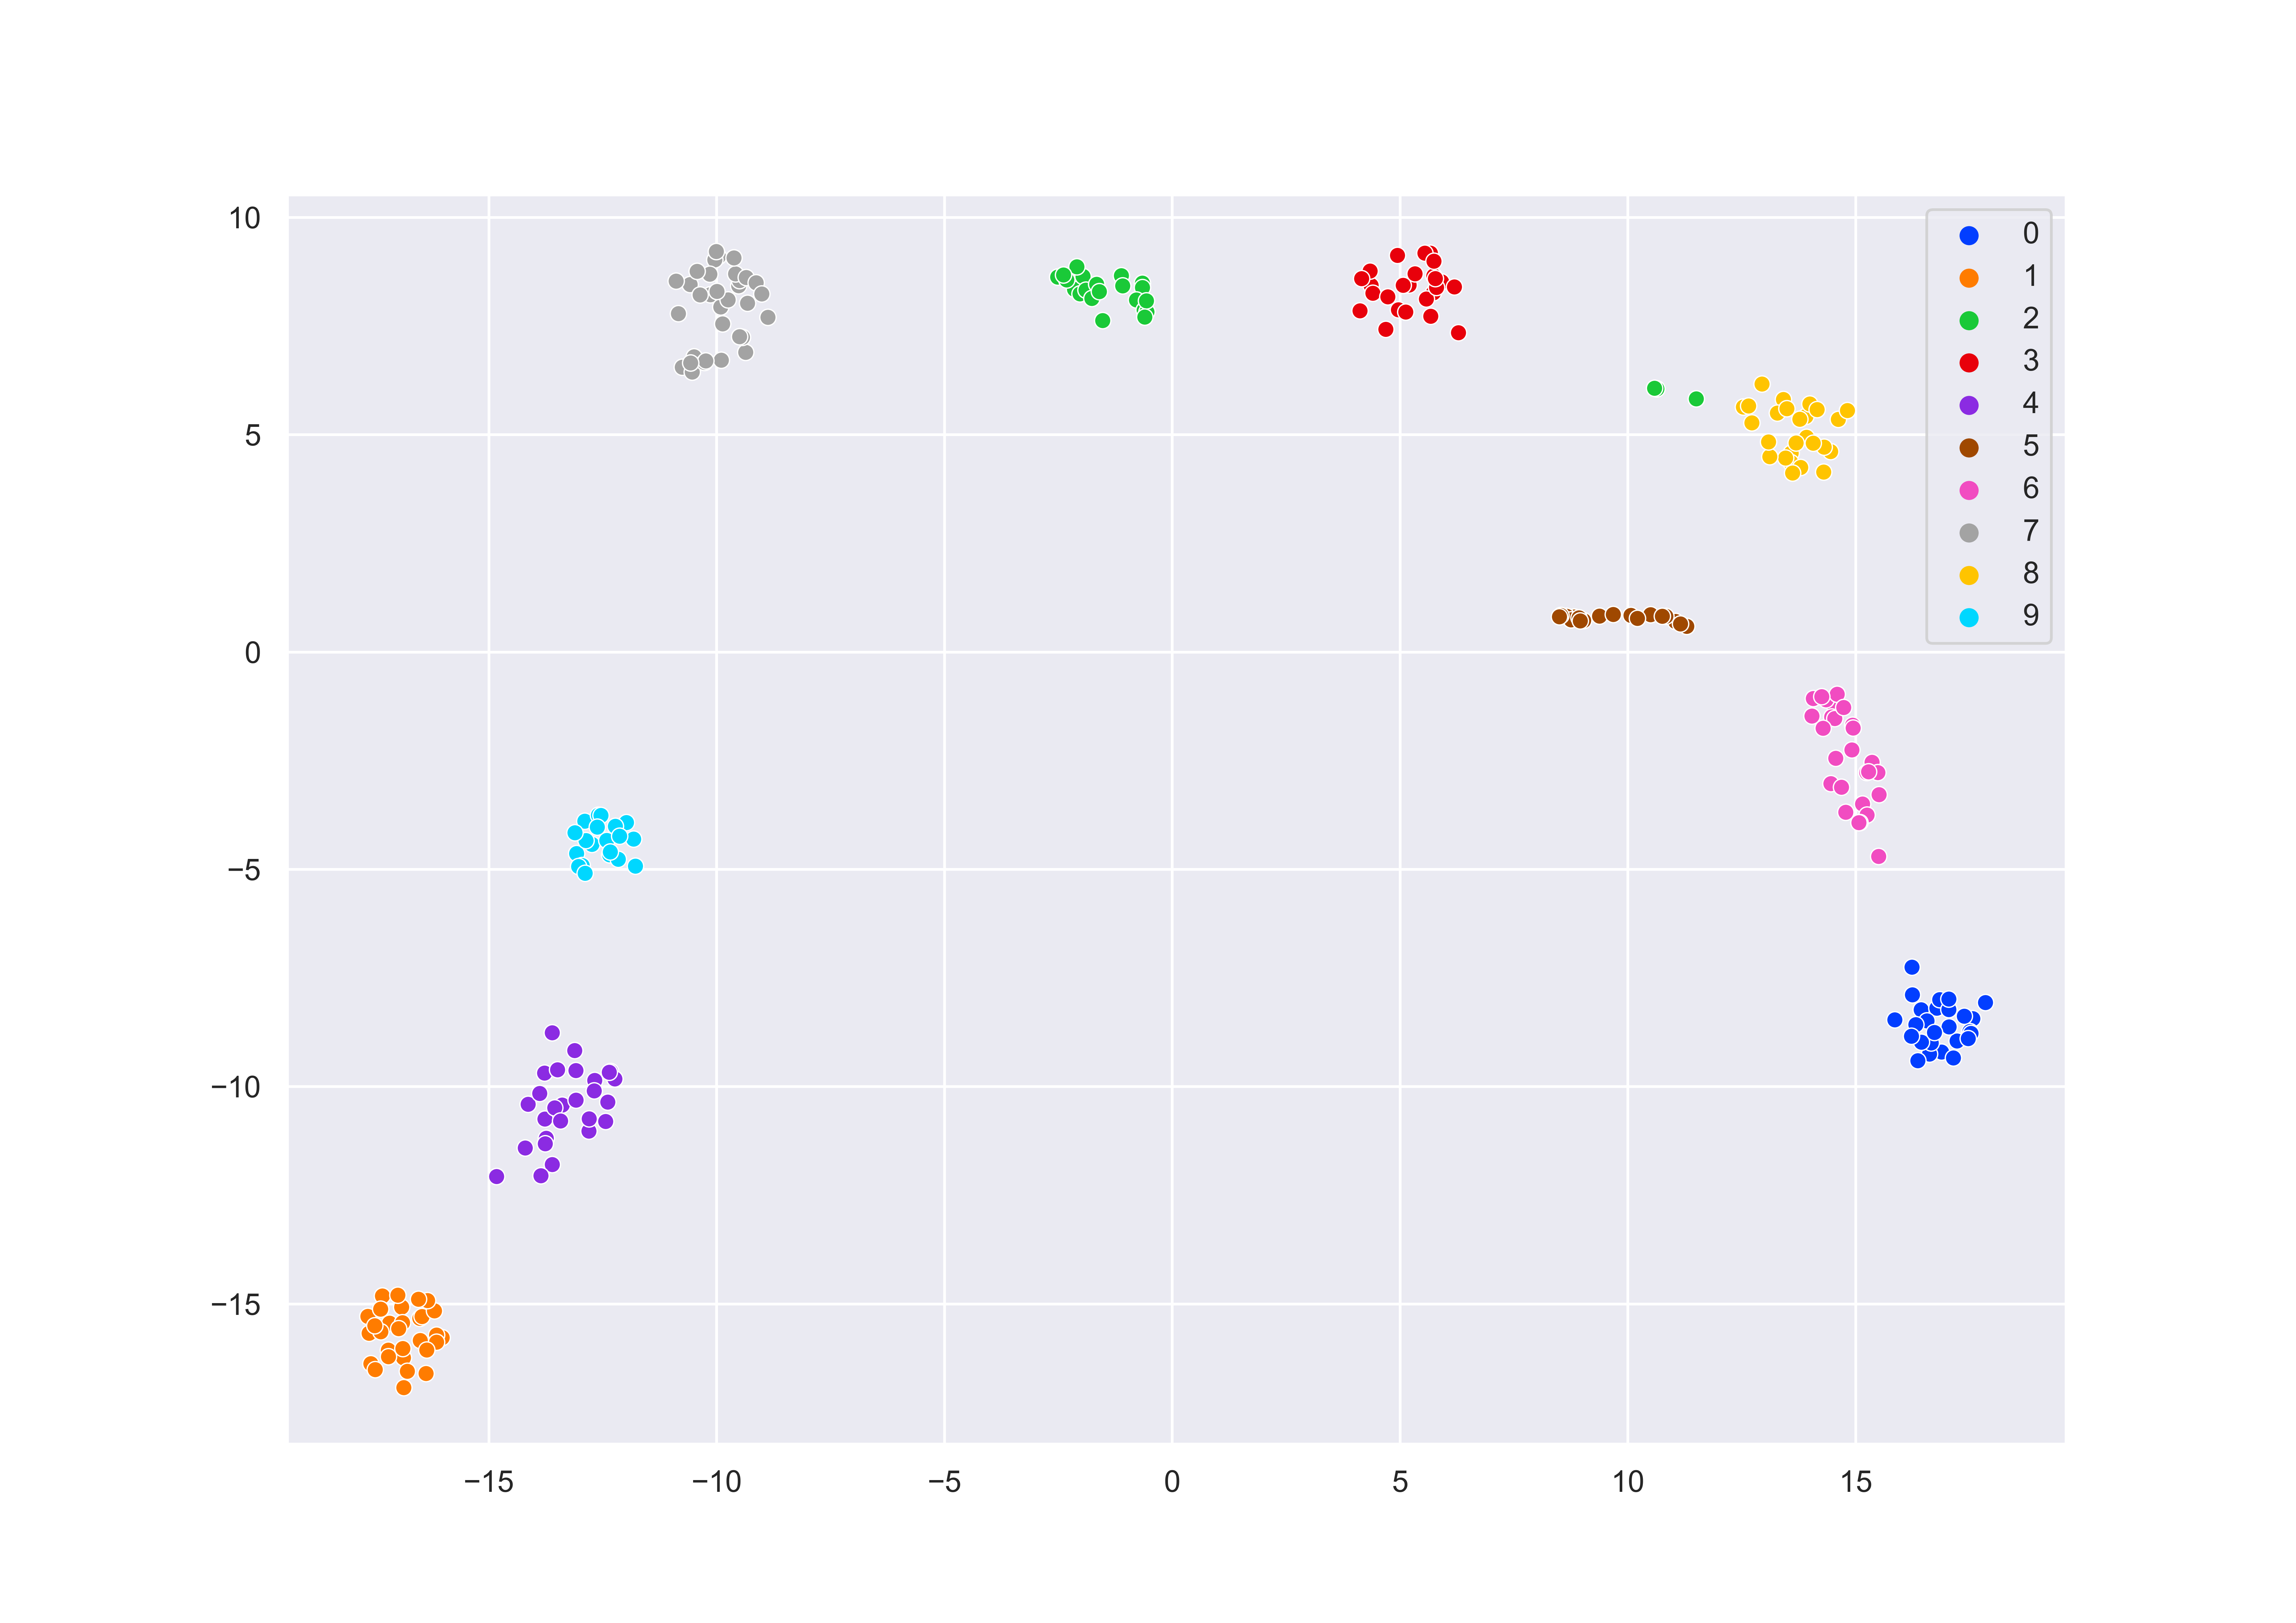
\includegraphics[width=0.32\linewidth]{../images/mnist_feature_map3_tsne.png}
        % \caption{Absolute value of indivisual components of weight in ridge regression when setting $\lambda$ to 1.5.}
        \label{fig:mnist_tSNE_3}
    \end{subfigure}
    \caption{Visualization images of intermediate output tensors with t-SNE method. Left: Tensors after the first max pooling layer. Middle: Tensors after the second max pooling layer. Right: Tensors after the output linear layer.}
    \label{fig:mnist_tsne}
\end{figure}
\section{Image Classification}

\subsection{Model \& Hyperparameters}
I design a 2-layer CNN models with an additional linear and softmax layer. The architecture can be interpreted in Fig.~\ref{fig:CNN_arch}. 
I set the batch size to 256 so as to maintain the high capability of batch normalization layer. 
The learning rate is set to 0.001 and the dropout rate is set to 0.1.
I train the whole model for 30 epochs and select the checkpoint with best binary cross entropy loss for evaluation on test set.

\subsection{Loss Function}
Because it is a classification task. I should have used cross entropy loss. 
But for training stability, I add an additional logarithm layer after the output softmax layer and use \verb|nn.LogSoftmax| instead of \verb|nn.Softmax| in pytorch.
So the loss function is simultaneously changed to negative log-liklihood loss.
\begin{equation}
    \label{eq:nllloss}
    \mathcal{L}=-\sum_{i}\sum_{k}y_k^*\cdot y_k
\end{equation}
where $k=1,2,\cdots, K$ and $K$ is the number of classes.

\subsection{Experiment Results}
The selected checkpoint can achieve $99.39\%$ accuracy in test set. The loss and accuracy change figures of self-designed CNN model are depicted in Fig.~\ref{fig:cnn_loss_acc}. It can be seen that the change is smooth, which proves that the hyperparameters are well-set and does not require more tuning steps.
\newline
\newline
\noindent 
Besides, I output the tensor after the first pooling layer, the tensor after the second pooling layer and the tensor after the output linear layer. 
And then I use PCA and t-SNE to respectively visualize them in order to see what my model has learned during training.
Their corresponding results are depicted in Fig.~\ref{fig:mnist_pca} and Fig.~\ref{fig:mnist_tsne}, respectively.
It can be seen that the first tensor cannot distinguish well each images but after the second CNN layer, my model has learned to distinguish each image with high accuracy.
The corresponding PCA code is presented below and the t-SNE code is pasted at the end of the report. 
I follow the handout of Prof. Zhang to implement it by myself.
My implemented PCA method does not use eigen-decomposition based method because it costs a lot. 
Instead, I use SVD to extract main components which can also represent the feature of original data. 
The code for SVD is shown below and the main structure of code of t-SNE is shown in Sec.~\ref{code:tsne}
\begin{lstlisting}
class MyPCA:
    def __init__(self, n_components: int = 2) -> None:
        self.n = n_components
    
    def fit(self, X: np.ndarray):
        n_samples, n_features = X.shape
        assert n_features >= self.n, "Main components must be less than or equal to total feature numbers"
        mean_val = X.mean(0, keepdims=True)
        X = X - mean_val
        U, sigma, VT = np.linalg.svd(X, False)
        self.P = U[:, :self.n]
        max_abs_cols = np.argmax(np.abs(U), axis=0)
        signs = np.sign(U[max_abs_cols, range(U.shape[1])])
        U *= signs
        VT *= signs[:, np.newaxis]
        self.P = VT[:self.n]

        return self
    
    def transform(self, X):
        return X @ self.P.T
\end{lstlisting}